\documentclass[border=3pt, 12pt]{standalone}

\usepackage{tikz}
\usetikzlibrary{shapes, arrows}
\usetikzlibrary{calc}

\tikzset{
%
data/.style={
% The shape:
rectangle,
% The size:
minimum width=25mm,
minimum height=10mm,
% The border:
very thick,
draw=black!80,
% fill
fill=gray!20
},%
%%%%%%%%%%
dummy/.style={%
draw=none,
fill=none%
},%
}

\begin{document}

\newcommand{\mltext}[2]{\begin{tabular}{c} #1 \\ #2 \end{tabular}}

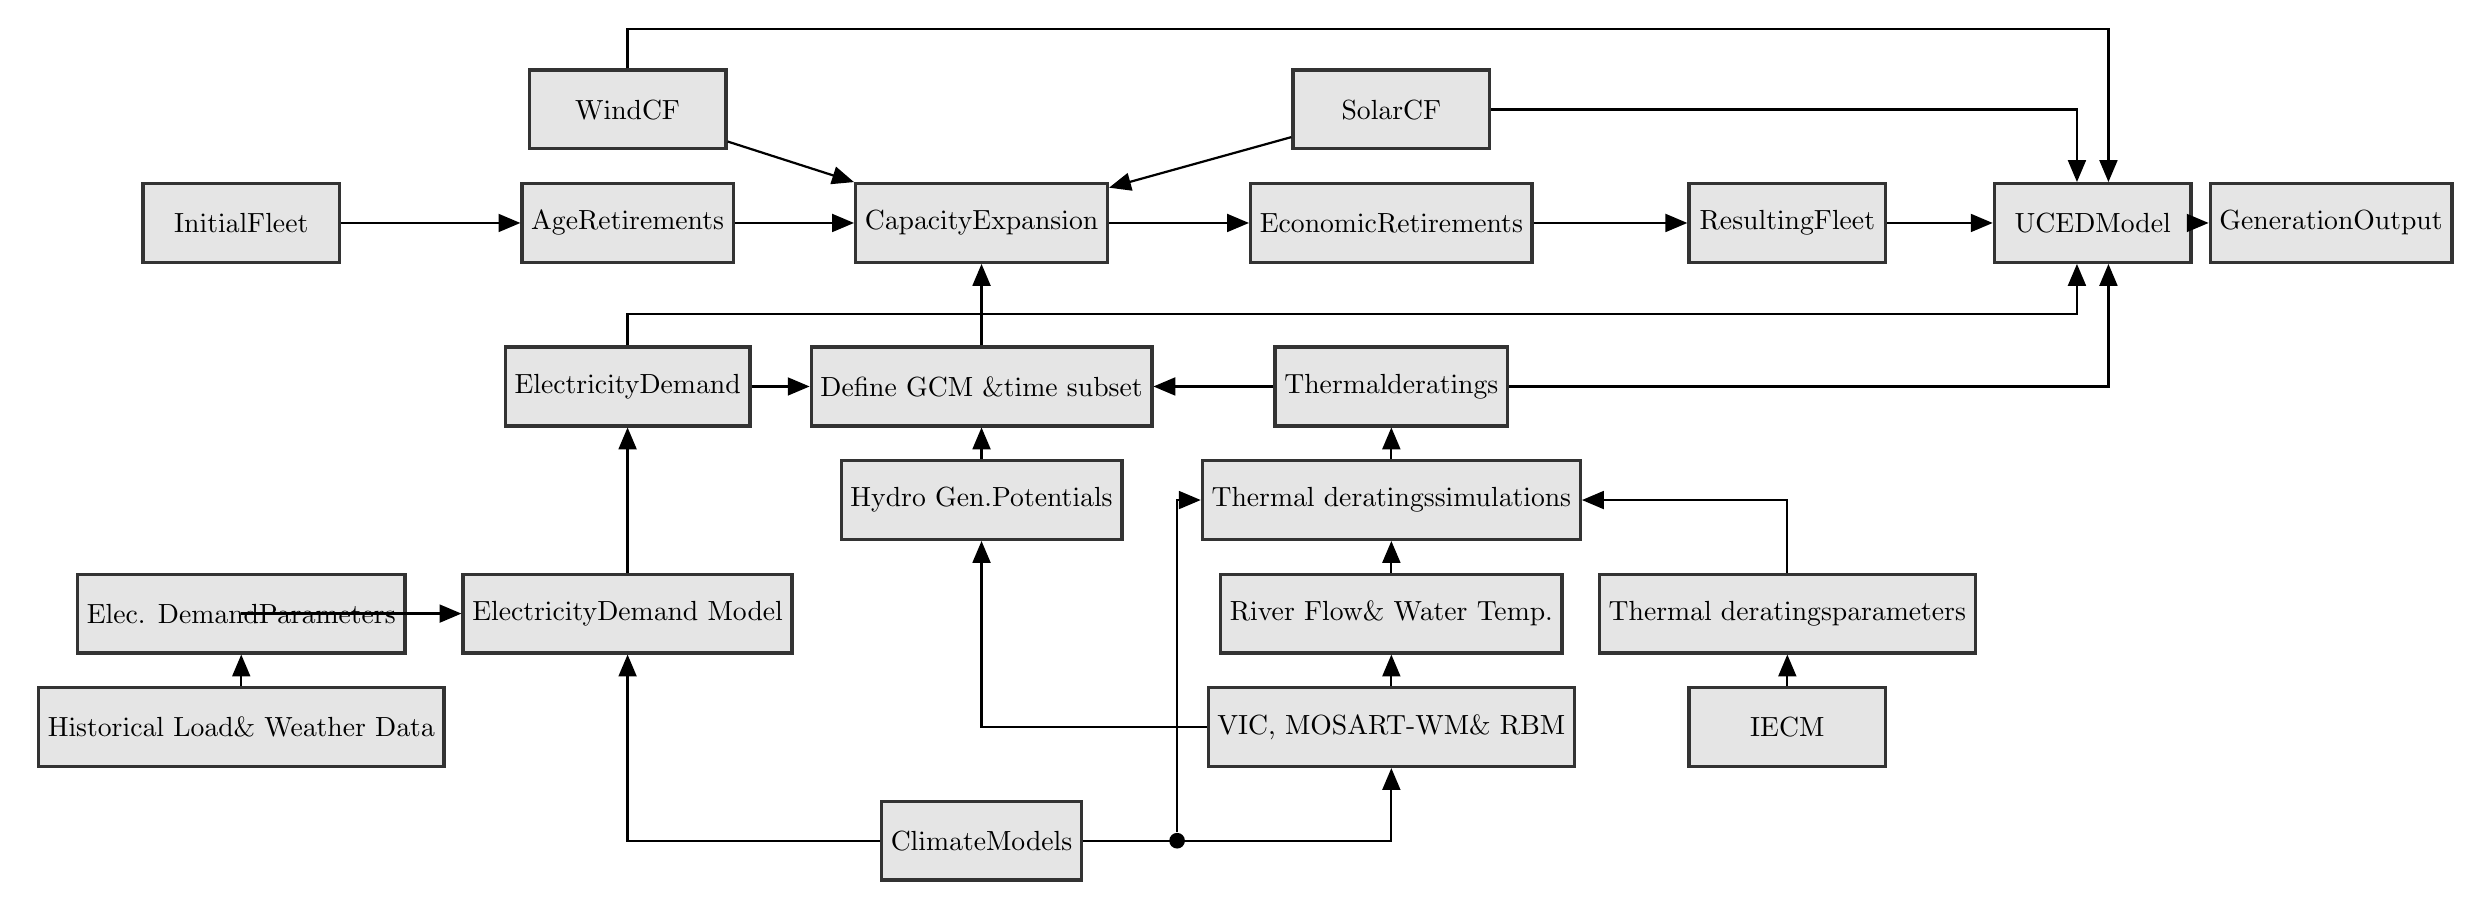
\begin{tikzpicture}

% auxiliary grid
%\draw[step=1cm, gray, very thin] (-18, -7) grid (18, 7);

\matrix[row sep=4mm, column sep=2mm]{
% "zero" row (just to add space)
& & \\
% row
 & \node [data]  (windcf) {\mltext{Wind}{CF}}; & & & \node [data]  (solarcf) {\mltext{Solar}{CF}}; \\
% row
\node [data] (initial fleet) {\mltext{Initial}{Fleet}};  &
\node [data]  (pre retire) {\mltext{Age}{Retirements}}; &
\node [data]  (ce) {\mltext{Capacity}{Expansion}}; &
&
\node [data]  (post retire) {\mltext{Economic}{Retirements}}; & 
\node [data] (final fleet) {\mltext{Resulting}{Fleet}}; &
\node [data] (uc) {\mltext{UCED}{Model}}; &
\node [data] (uc result) {\mltext{Generation}{Output}};
\\
% EMPTY ROW (just to add space for edges crossing to UC model)
&  & \node [dummy] (dummy2) {\mltext{ }{ }};\\
% rows
&  \node [data] (demand) {\mltext{Electricity}{Demand}}; & \node [data] (getscenarios) {\mltext{Define GCM \&}{time subset}}; & & \node [data] (curtail) {\mltext{Thermal}{deratings}};\\
% row
&  &  \node [data] (hydropot) {\mltext{Hydro Gen.}{Potentials}}; & & \node [data] (curtailregression) {\mltext{Thermal deratings}{simulations}}; \\
% row
\node [data] (demandmodelparam) {\mltext{Elec. Demand}{Parameters}}; & \node [data] (demandmodel) {\mltext{Electricity}{Demand Model}}; & & & \node [data] (waterdata) {\mltext{River Flow}{\& Water Temp.}}; & \node [data] (curtailregressionparam) {\mltext{Thermal deratings}{parameters}};\\
% row
\node [data] (histdata) {\mltext{Historical Load}{\& Weather Data}}; & & & & \node [data] (uw) {\mltext{VIC, MOSART-WM}{\& RBM}}; & \node [data] (iecm) {IECM};\\
% row
& & \node [data] (gcms) {\mltext{Climate}{Models}}; &  \node [circle, fill=black, inner sep=2pt] (dummy1) {};\\
};
%
%
% Edges
\path[-triangle 45, thick]  	(windcf) edge (ce)
					(solarcf) edge (ce)				
					(initial fleet) edge (pre retire) 
					(pre retire) edge (ce)
					(ce) edge (post retire)
					(post retire) edge (final fleet)
					(demand) edge (getscenarios)
					(curtail) edge (getscenarios)
					(hydropot) edge (getscenarios)
					(getscenarios) edge (ce)
					(histdata) edge (demandmodelparam)					
					(demandmodel) edge (demand)
					(curtailregression) edge (curtail)
					(uw) edge (waterdata)
					(waterdata) edge (curtailregression)
					(final fleet)	 edge (uc)
					(uc) edge (uc result)
					(iecm) edge (curtailregressionparam);

\draw[->,-triangle 45, thick]	(dummy1) |- (curtailregression.west);
\draw[->,-triangle 45, thick] 	(uw.west) -| (hydropot.south);

\draw [->,-triangle 45, thick] (windcf.north)
% Now go up
-- ++(0,5mm)
% and go right and down
-| ($ (uc.north) + (2mm,0) $);

\draw[->,-triangle 45, thick]	(solarcf.east) -| ($(uc.north) - (2mm, 0)$);

\draw [->,-triangle 45, thick] (demand.north)
% Now go up
-- ++(0,4mm)
% and go right and down
-| ($ (uc.south) - (2mm,0) $);

\draw[->,-triangle 45, thick]	(curtail.east) -| ($(uc.south) + (2mm, 0)$);

\draw[->,-triangle 45, thick]	(gcms.west) -| (demandmodel.south);

\draw[->,-triangle 45, thick]	(gcms.east) -| (uw.south);
\draw[->,-triangle 45, thick]	(curtailregressionparam) |- (curtailregression);
\draw[->,-triangle 45, thick]	(demandmodelparam) |- (demandmodel);

\end{tikzpicture}

\end{document}  